\chapter{Simulator description}\label{chapt:simdescr}
\section{Introduction}
This chapter discusses in detail the different components of \gls{dfts}.

\section{Intermediate feature tensor packetization} \label{sec:simdescr:pkt}
A feature tensor with height $h$, width $w$, and the number of channels $c$ will be denoted $\gls{xtensor} \in \mathbb{R}^{\gls{h} \times \gls{w} \times \gls{c}}$. An illustration of a feature tensor extracted from layer \texttt{add\_1} of \gls{resnet18} \cite{ResNet} is shown in Fig. \ref{fig:simdescr:pkt:tensorviz}.
Layer \texttt{add\_1} corresponds to the output of the shortcut connection and element-wise addition applied to the final output of the \texttt{conv2\_x} layers, as denoted in \cite[Table 1]{ResNet}. Each channel in a DFTS2 tensor is partitioned into groups of $\gls{rpp}$ rows, as indicated by the dashed green lines in Fig. \ref{fig:simdescr:pkt:tensorviz}. Zero padding is done on the last packet of a channel if the number of channel rows ($\gls{h}$) is not an integer multiple of the number of packet rows ($\gls{rpp}$). Packetized tensors can be min-max quantized \cite{choi2018deep} to a user-specified number of bits/element. While it is possible to further compress the data packets by entropy coding, this was not implemented in the current version of DFTS  because the focus is on error resilience, not on compression.

\begin{figure}[H]
	\centering
	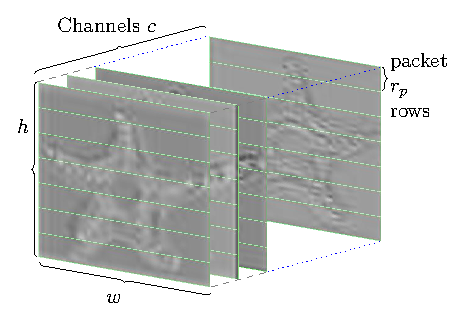
\includegraphics[scale=1]{Figures/tensorlostviz3icip.pdf}
	\caption[ResNet18 tensor visualization]{A tensor $\mathcal{X} \in \mathbb{R}^{h \times w \times c}$ from layer \texttt{add\_1} of ResNet-18. Several consecutive rows in each channel form a feature data packet.}
	\label{fig:simdescr:pkt:tensorviz}
\end{figure}

In \verb|yaml| files, the packetization parameter may be specified as shown below
\verbatiminput{Files/pktexample.yml}
Packetization is implemented in \verb|models.packetModel.py|. The user can create a packetization object with the following code snippet. The \verb|rowsPerPacket| is the desired number of rows per packet \gls{rpp} for each feature tensor channel. \verb|deviceOut| is a deep feature tensor \gls{xtensor}, usually output by the device sub-model.

\begin{lstlisting}[language=Python, caption=Creating a packetization object]
	from models.packetModel import PacketModel as PacketModel
	pkt_obj_model = PacketModel(rows_per_packet=rowsPerPacket,
	data_tensor=deviceOut)
\end{lstlisting}

The packetized tensor data may be accessed as

\begin{lstlisting}[language=Python, caption=Manipulating packetized tensor data]
	packetized_data = pkt_obj_model.packet_seq
	unpacketized_data = pkt_obj_model.data_tensor
\end{lstlisting}

In \verb|add_1| \gls{resnet18} tensors, there are 64 channels, each of which is $56 \times 56$. With $\gls{rpp}=8$, we have 7 packets of $8 \times 56$ elements each. So \verb|packetized_data| would be a 32-bit floating point \verb|numpy| array of dimensions $7 \times 8 \times 56 \times 64$. When dealing with tensor data for a batch of $k$ images, then \verb|packetized_data| would be $k \times 7 \times 8 \times 56 \times 64$. \verb|unpacketized_data| would be $k \times 56 \times 56 \times 64$. 


\section{Channel models} \label{sec:simdescr:channel}
DFTS offers three models for the communication channel model: random loss, i.e., independent and identically distributed (iid), Gilbert-Elliott and external packet traces. Technically, the perfect channel model case, that is, no packet loss at all, is also a channel model.

In \verb|yaml| files, the communication channel parameters may be specified as shown below.
\verbatiminput{Files/channelexample.yml}
The user can switch between channel models by editing the \verb|include| flag. If no channel model is selected (all three \verb|include| flags are \verb|False|), the \gls{dfts} experiment will be run in the perfect channel model mode. 

Gilbert and random loss channel models are implemented in \verb|gbChannel.py| and \verb|trivialChannel.py| in the \verb|channel| directory. An object may be initialized for these two models using the following code snippet. \verb|channel| is a dictionary created by processing the \verb|yaml| file.

\begin{lstlisting}[language=Python,caption=Creating a lossy channel model object]
	from runExpt.calloc import loadChannel
	channel = loadChannel(channel)
\end{lstlisting}
The \verb|channel| object is then passed to the function \verb|transmit| which unsurprisingly transmits the packetized bitstream over a lossy channel.

\begin{lstlisting}[language=Python,caption=Lossy channel model]
	from .simmods import *
	dO, lM, rI, lI = transmit(deviceOut, channel, rowsPerPacket)
\end{lstlisting}

\verb|deviceOut| is the device sub-model output tensor (may or may not be quantized). \verb|d0| is the packetized (according to \verb|rowsPerPacket|-\gls{rpp}) tensor transmitted over an unreliable \verb|channel| realization. \verb|lM| is the loss matrix, \verb|rI| is a list of received indices while \verb|lI| is a list of lost indices.

We will later on discuss how the user should go about loading external packet traces.

\subsection{Gilbert-Elliott channels}

\subsection{Packet traces}

\section{Packet loss concealment} \label{sec:simdescr:ec}
By recovering missing packets in deep feature tensors, we are able to provide the cloud sub-model with more ``complete" tensor data to exploit in order to complete the inference task. \gls{dfts} allows the user to switch on or off error concealment. The following packet loss concealment methods include
\begin{itemize}
	\item general tensor completion methods: \gls{silrtc} \cite{liu2012tensor} and \gls{halrtc} \cite{liu2012tensor}.\\
	These methods were developed to recover missing values in visual data. They make no assumption as to the nature of the loss (in other words, they are agnostic to the chosen packetization scheme). \gls{silrtc} and \gls{halrtc} adopt an iterative approach: they have to be run a number of times on the corrupted tensor to recover the missing packets. The number of iterations to be run is a parameter for the engineer to tune.
	\item methods which are specific to deep feature tensors in \gls{ci}: \gls{altec} \cite{Bragile2020} and \gls{caltec} \cite{CALTeC_ICIP_2021}. \\ \gls{altec} was originally developed for a single row of feature data per packet scheme. \gls{dfts} provides an \gls{altec} modified to handle a multiple rows of feature tensor data per packet scheme.
	\item image inpainting-based methods, such as Navier-Stokes \cite{navierstokes} which has been used for error concealment in \gls{ci} in \cite{Bajic2021objdet}.
\end{itemize}

\section{Simulation mode} \label{sec:simdescr:simmode}